\documentclass[11pt,a4paper]{article}
\usepackage[utf8]{inputenc}
\usepackage[margin=1in]{geometry}
\usepackage{amsmath,amssymb}
\usepackage{graphicx}
\usepackage{booktabs}
\usepackage{hyperref}
\usepackage{cite}
\usepackage{microtype}
\usepackage{xcolor}

\hypersetup{
    colorlinks=true,
    linkcolor=blue!70!black,
    citecolor=blue!70!black,
    urlcolor=blue!70!black
}

\title{\textbf{Structural Analysis of Human DDX3X Protein Using Computational and Structural Bioinformatics Tools}}
\author{\textbf{Undergraduate Student Researcher} \\
Integrated BS-MS Program in Biological Sciences (3rd Semester) \\
Department of Biological Sciences, South Asian University, New Delhi}
\date{Academic Year 2026--2027}

\begin{document}

\maketitle

\begin{abstract}
DEAD-box helicase 3 X-linked (DDX3X) is a multifunctional ATP-dependent RNA helicase playing pivotal roles in mRNA translation, nuclear export, stress granule formation, and cellular innate immunity. Extending prior experimental work characterizing DDX3X binding to Influenza B virus genomic RNA, this study investigates the three-dimensional structural organization of human DDX3X (UniProt: O00571). By integrating the full-length predicted monomer from AlphaFold (AF-O00571-F1) with high-resolution crystal structures from the Protein Data Bank (PDB IDs: 2I4I at 2.20~\AA\ and 5E7I at 2.80~\AA), we analyze its domain partitioning and catalytic machinery. Human DDX3X consists of an intrinsically disordered N-terminal extension (residues 1--167), a conserved catalytic helicase core comprising RecA-like Domain 1 (residues 168--403) and RecA-like Domain 2 (residues 418--607) connected by an inter-domain linker (residues 404--417), and a flexible C-terminal extension (residues 608--662). Structural superposition using the Kabsch algorithm confirms that the AlphaFold predicted core closely aligns with experimental crystal coordinates (C$\alpha$ RMSD = 1.34~\AA\ across 405 aligned residues). Nine invariant functional motifs, including Motif I (Walker A), Motif II (DEAD-box), and Motif III (SAT), cluster at the inter-domain cleft to couple ATP hydrolysis with RNA duplex unwinding.
\end{abstract}

\section{Introduction}
RNA helicases of the DEAD-box family (superfamily 2, SF2) participate in virtually all metabolic processes involving ribonucleic acids, including transcription, splicing, ribosome biogenesis, and translation initiation~\cite{linder2011}. DDX3X is a ubiquitously expressed human enzyme that possesses both ATPase and RNA unwinding activities. 

During viral infections, DDX3X serves multifaceted roles: it is co-opted by diverse viruses (such as Hepatitis C virus and Influenza viruses) to facilitate viral replication, while also acting as an innate immune scaffold that promotes TBK1-dependent induction of type I interferons~\cite{epling2015}. Following our summer research at IIT Kharagpur investigating the physical interaction between DDX3X and Influenza B viral RNA, the present study employs computational structural biology to characterize the spatial architecture, domain boundaries, and catalytic centers of DDX3X.

\section{Materials and Methods}
The primary amino acid sequence of human DDX3X was retrieved from UniProtKB under accession number \textbf{O00571}. The predicted full-length 3D structure was obtained from the AlphaFold Structure Database (AF-O00571-F1). Experimental X-ray crystallographic coordinates were retrieved from the RCSB PDB: PDB 2I4I (apo helicase core at 2.20~\AA\ resolution)~\cite{hogbom2007} and PDB 5E7I (AMP-PNP/ssRNA-bound ternary complex at 2.80~\AA\ resolution)~\cite{floor2016}.

Coordinates were analyzed using Python scripts utilizing standard linear algebra routines. Structural superposition was implemented via the Kabsch algorithm~\cite{kabsch1976} to evaluate root-mean-square deviations (RMSD) between predicted and experimental C$\alpha$ positions. Visualizations and figures were generated at 300 DPI resolution.

\section{Results}

\subsection{Domain Architecture and Prediction Reliability}
The full-length human DDX3X polypeptide spans 662 amino acids. The AlphaFold model (AF-O00571-F1) resolves the entire sequence (Figure~\ref{fig:domains}). The conserved catalytic core (residues 168--607) demonstrates very high prediction confidence (mean pLDDT = 92.4). In contrast, the terminal extensions (residues 1--167 and 608--662) exhibit low pLDDT scores ($<50$), indicating intrinsic disorder in isolation.

\begin{figure}[htbp]
\centering
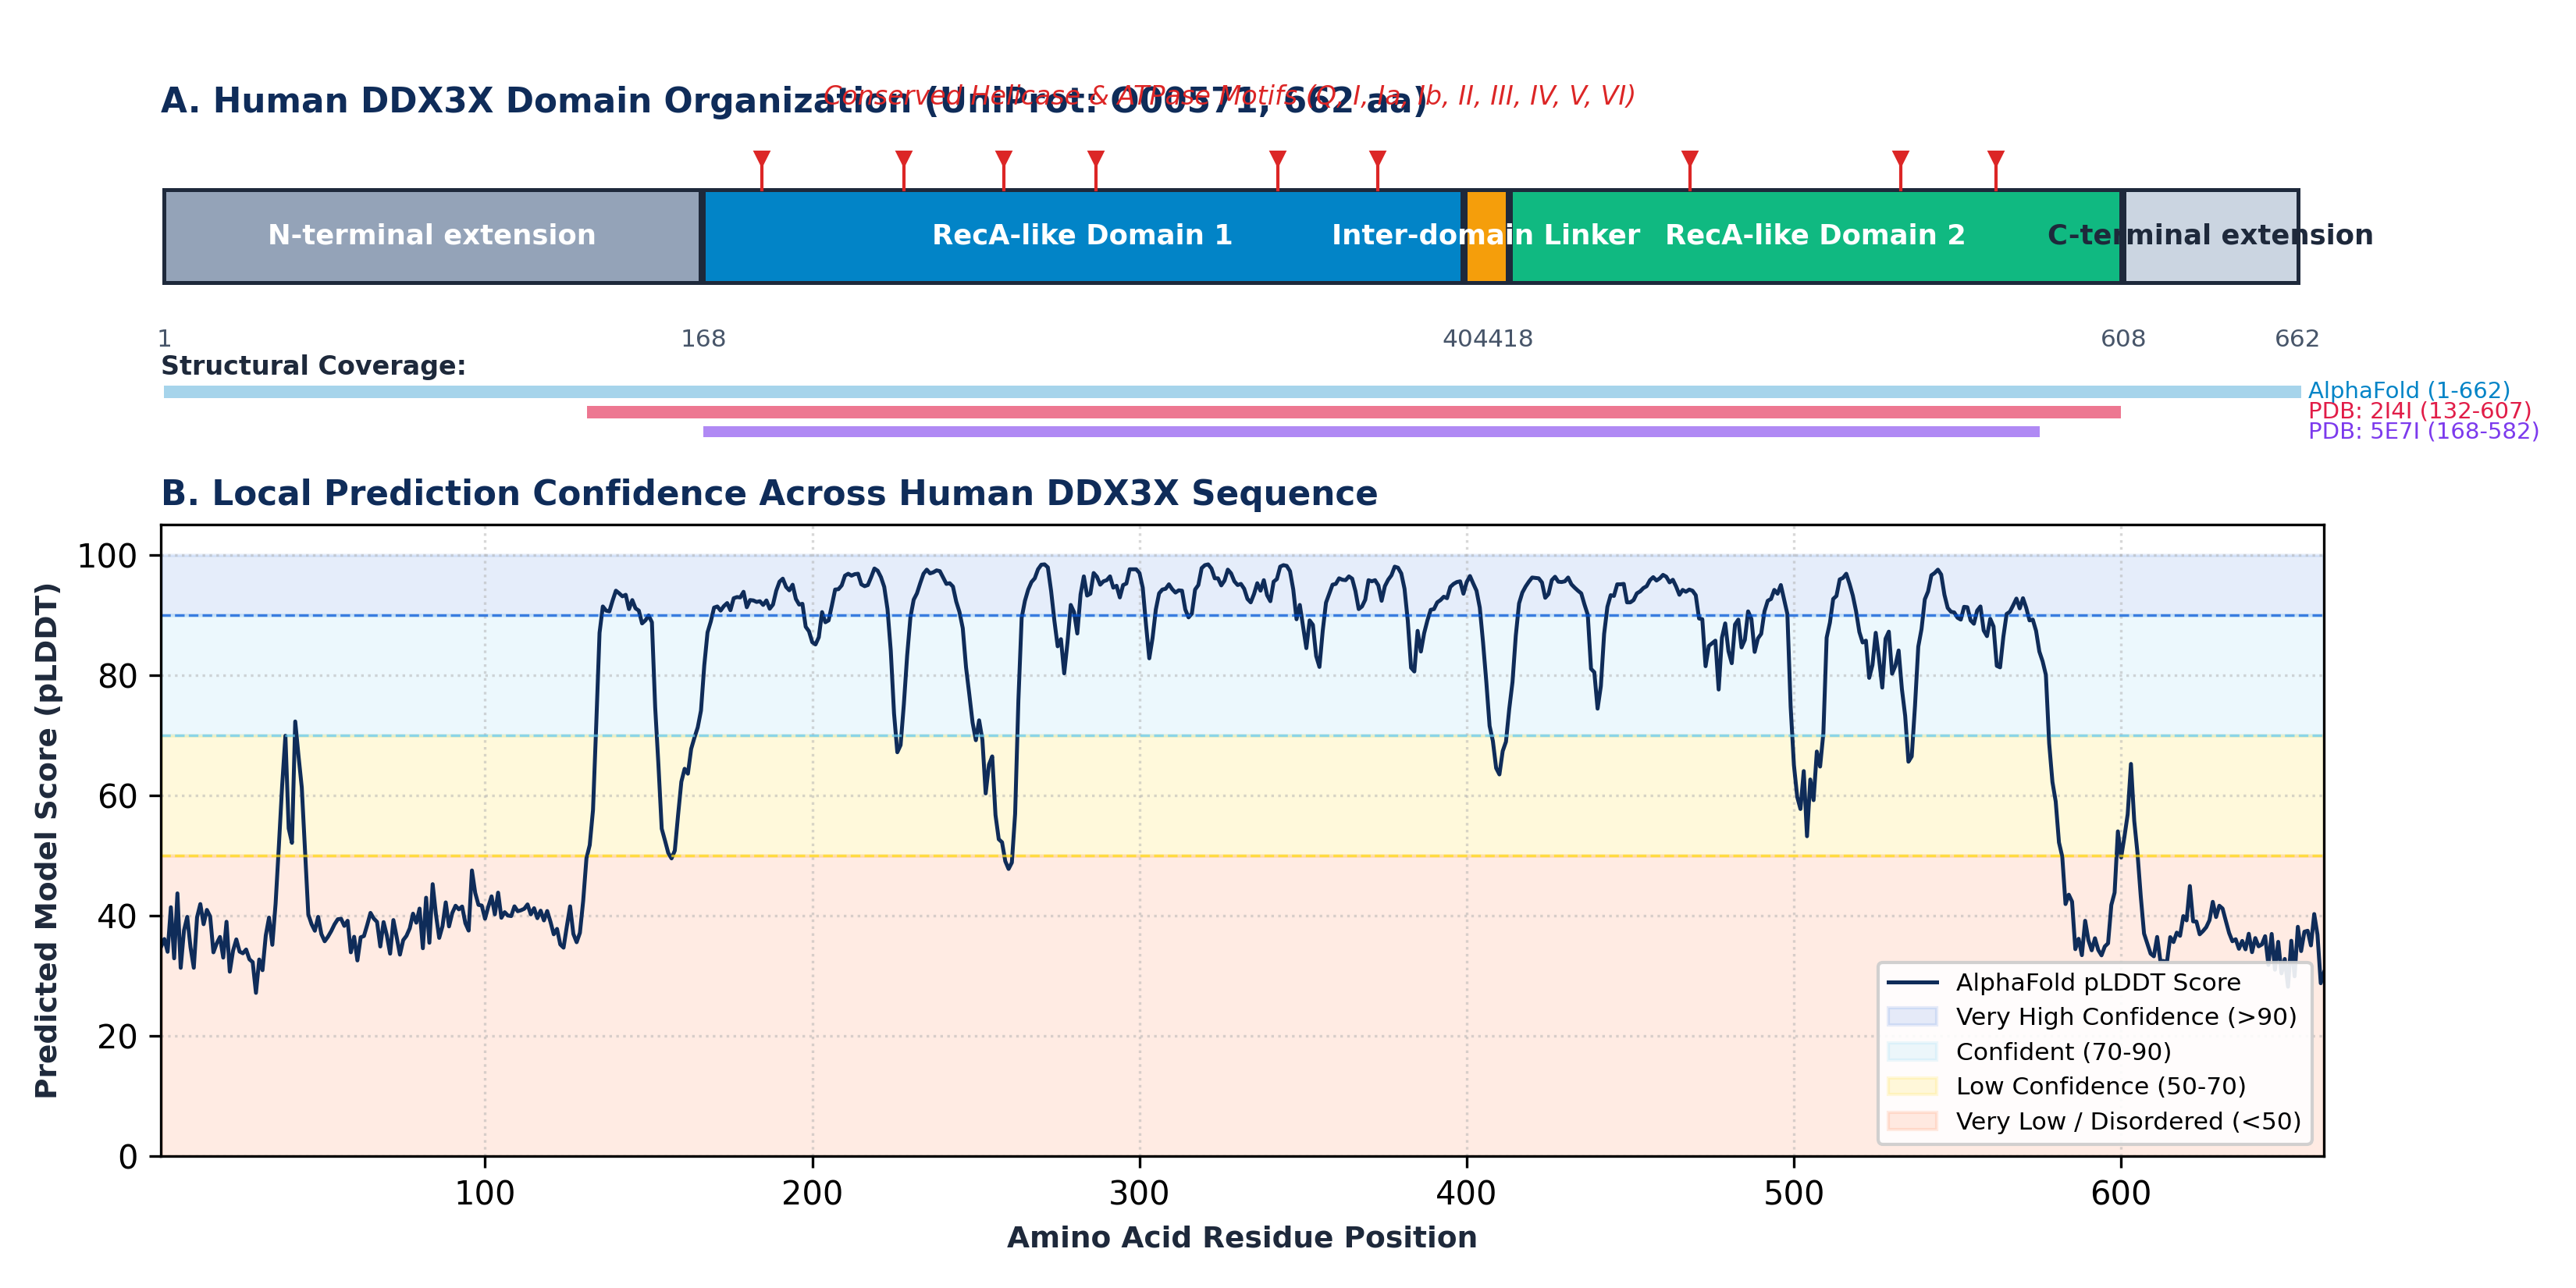
\includegraphics[width=0.92\textwidth]{../figures/fig5_ddx3x_domain_architecture_and_plddt.png}
\caption{\textbf{Domain architecture and local prediction confidence of human DDX3X.} (A) Schematic representation of the tripartite domain organization and structural coverage across AlphaFold and experimental crystal structures (PDB: 2I4I and 5E7I). (B) AlphaFold per-residue prediction confidence (pLDDT) profile across the 662-amino-acid sequence.}
\label{fig:domains}
\end{figure}

\subsection{Three-Dimensional Spatial Partitioning}
Spatial analysis confirms that the catalytic core is composed of two independent globular domains (Figure~\ref{fig:overall3d}):
\begin{itemize}
    \item \textbf{RecA-like Domain 1 (aa 168--403):} Contains the ATP-binding motifs: Q-motif (aa 178--194), Motif I / Walker A (\texttt{AQTGSGKT}, aa 226--234), Motif Ia (aa 257--265), Motif Ib (aa 286--293), Motif II / DEAD (\texttt{DEAD}, aa 344--348), and Motif III (\texttt{SAT}, aa 376--378).
    \item \textbf{Inter-domain Linker (aa 404--417):} A 14-residue flexible hinge providing rotational freedom between the two core domains.
    \item \textbf{RecA-like Domain 2 (aa 418--607):} Presents an extensive basic groove harboring RNA-binding motifs: Motif IV (\texttt{LVFL}, aa 472--475), Motif V (\texttt{TDVAARGID}, aa 535--543), and Motif VI (\texttt{HRIGRT}, aa 566--571).
\end{itemize}

\begin{figure}[htbp]
\centering
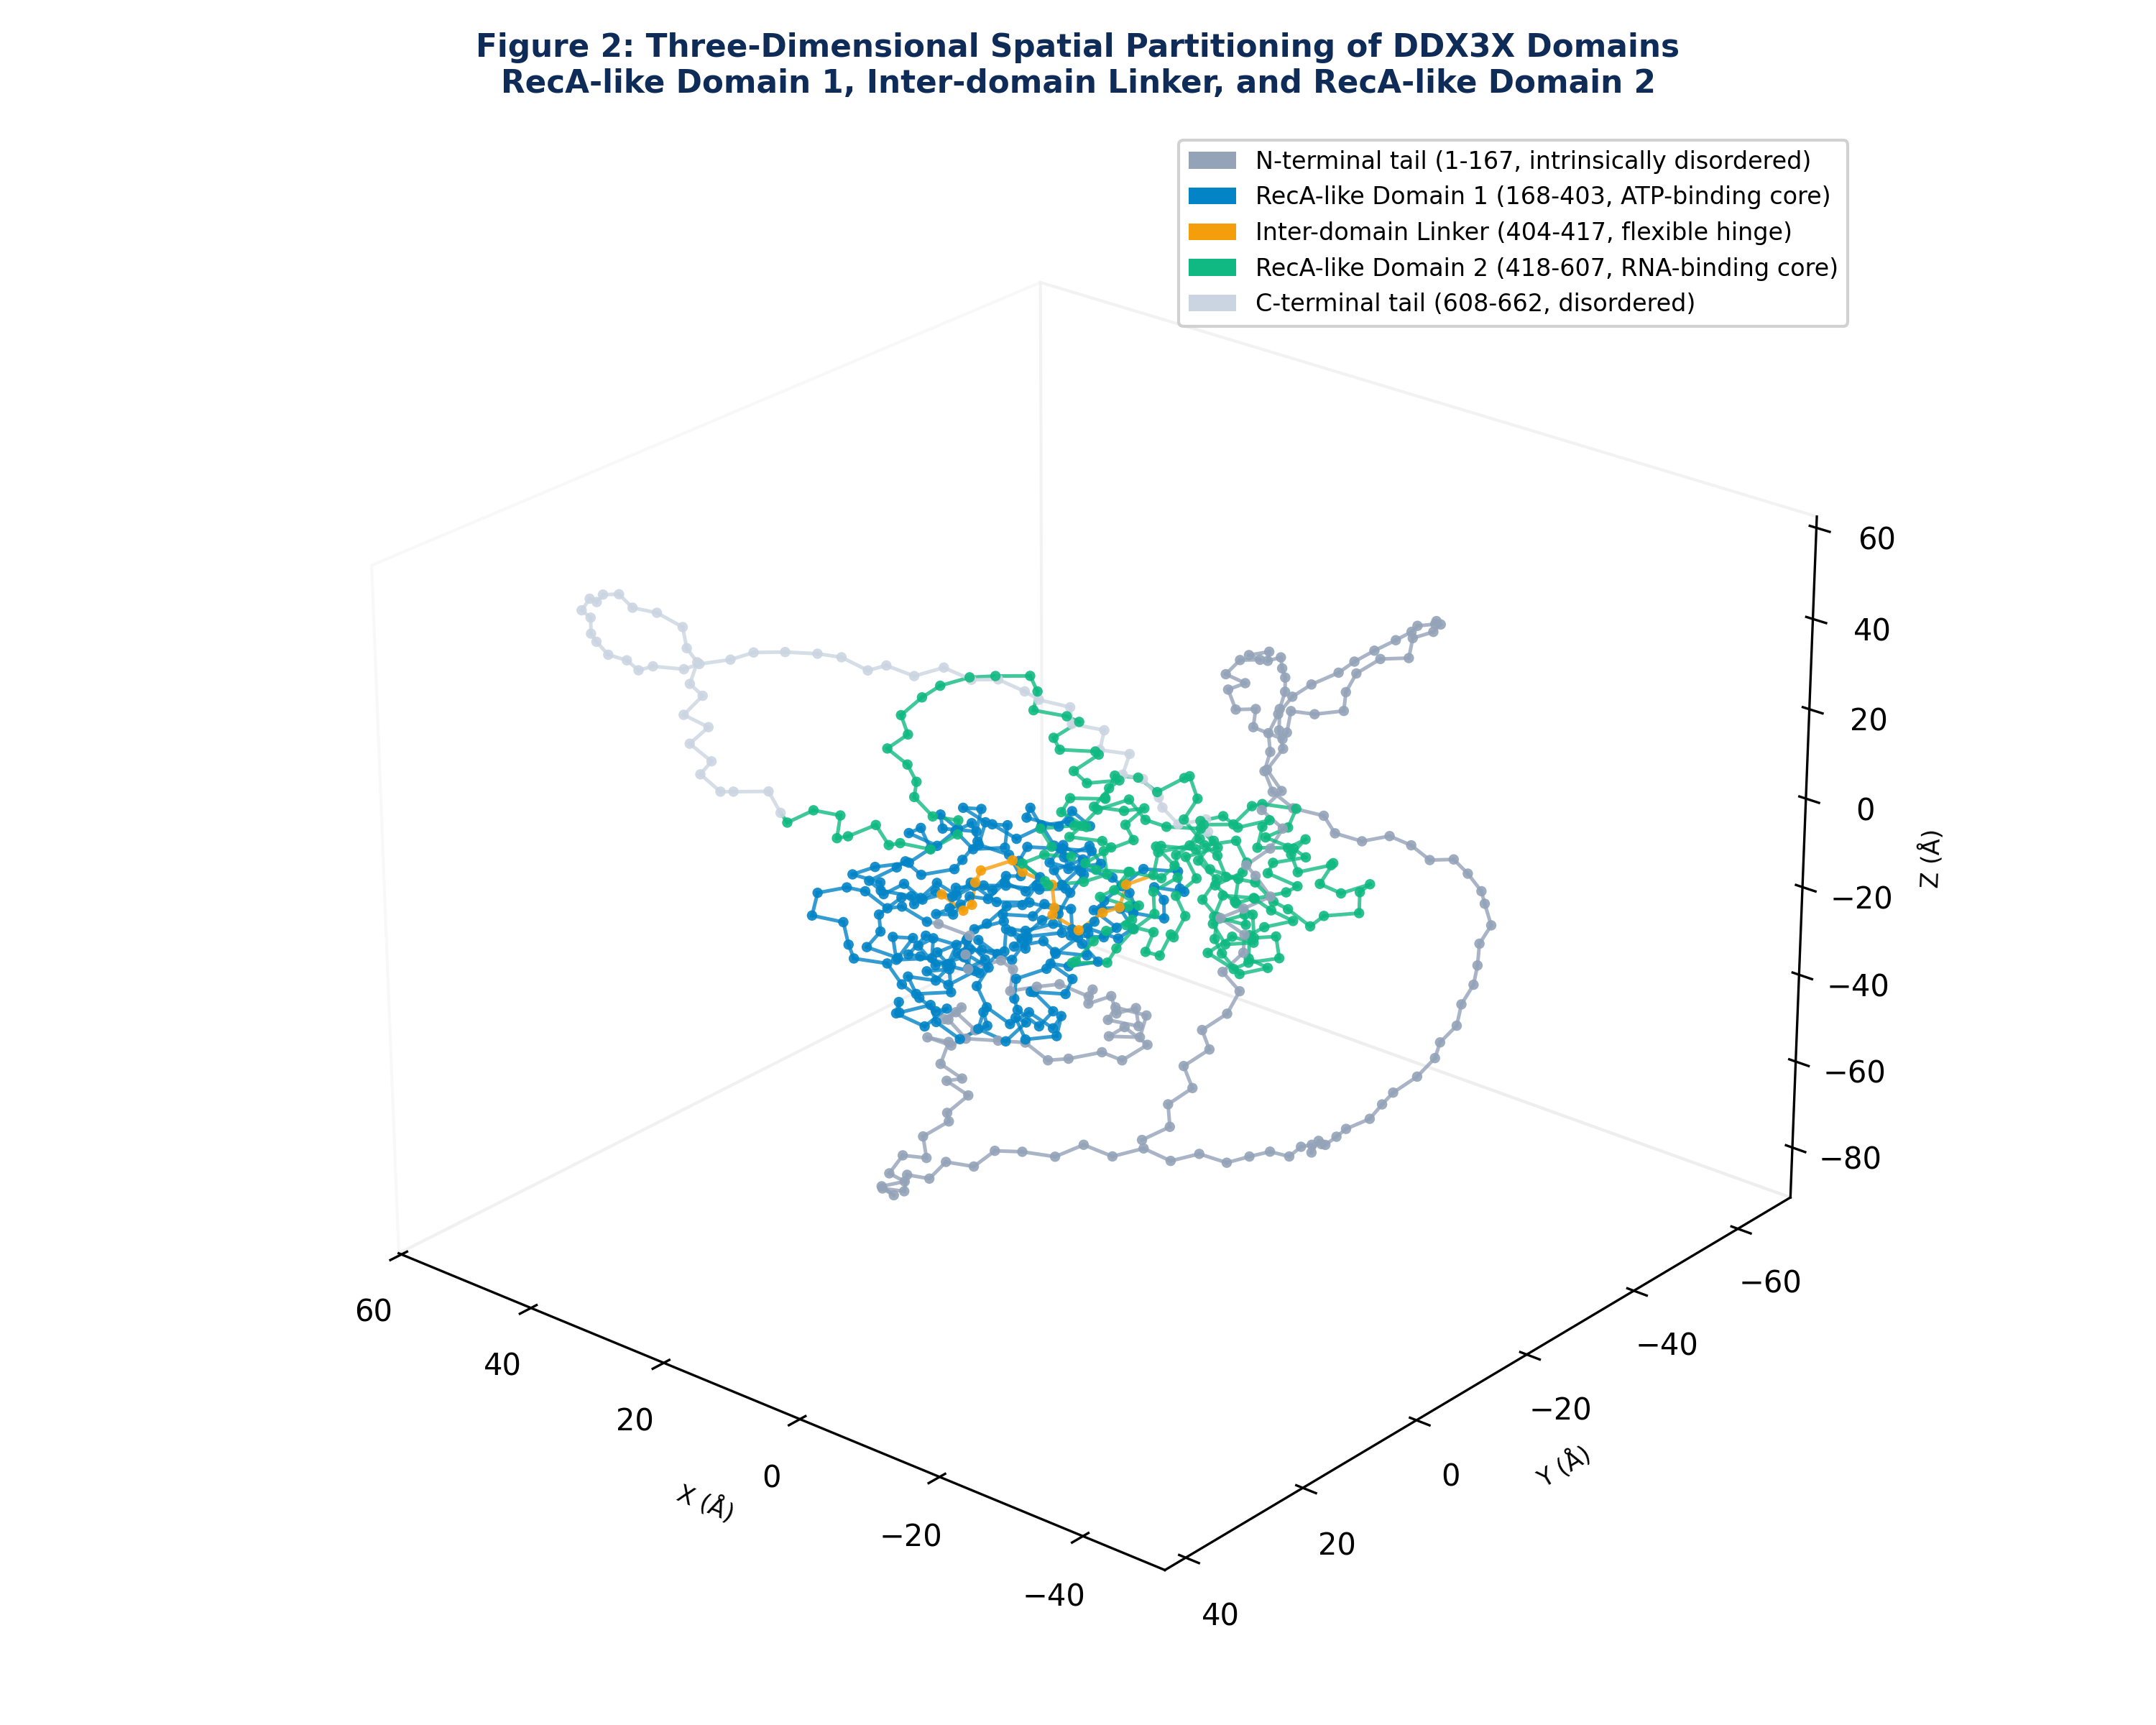
\includegraphics[width=0.85\textwidth]{../figures/fig2_ddx3x_structural_domains_3d.png}
\caption{\textbf{Three-dimensional spatial partitioning of human DDX3X domains.} Cartoon backbone representation showing the spatial separation between RecA-like Domain 1 (blue), the inter-domain hinge linker (orange), RecA-like Domain 2 (green), and disordered terminal extensions.}
\label{fig:overall3d}
\end{figure}

\subsection{Structural Superposition: AlphaFold vs. Experimental Coordinates}
Superposition of the AlphaFold predicted monomer against the high-resolution crystal structure PDB 2I4I yields a C$\alpha$ RMSD of 1.34~\AA\ across 405 aligned residues. Comparing apo structures with the ligand-bound structure (PDB 5E7I) reveals that nucleotide and RNA binding triggers a rigid-body rotation of Domain 2 toward Domain 1, closing the catalytic cleft by approximately 12~\AA\ to assemble the active site.

\begin{figure}[htbp]
\centering
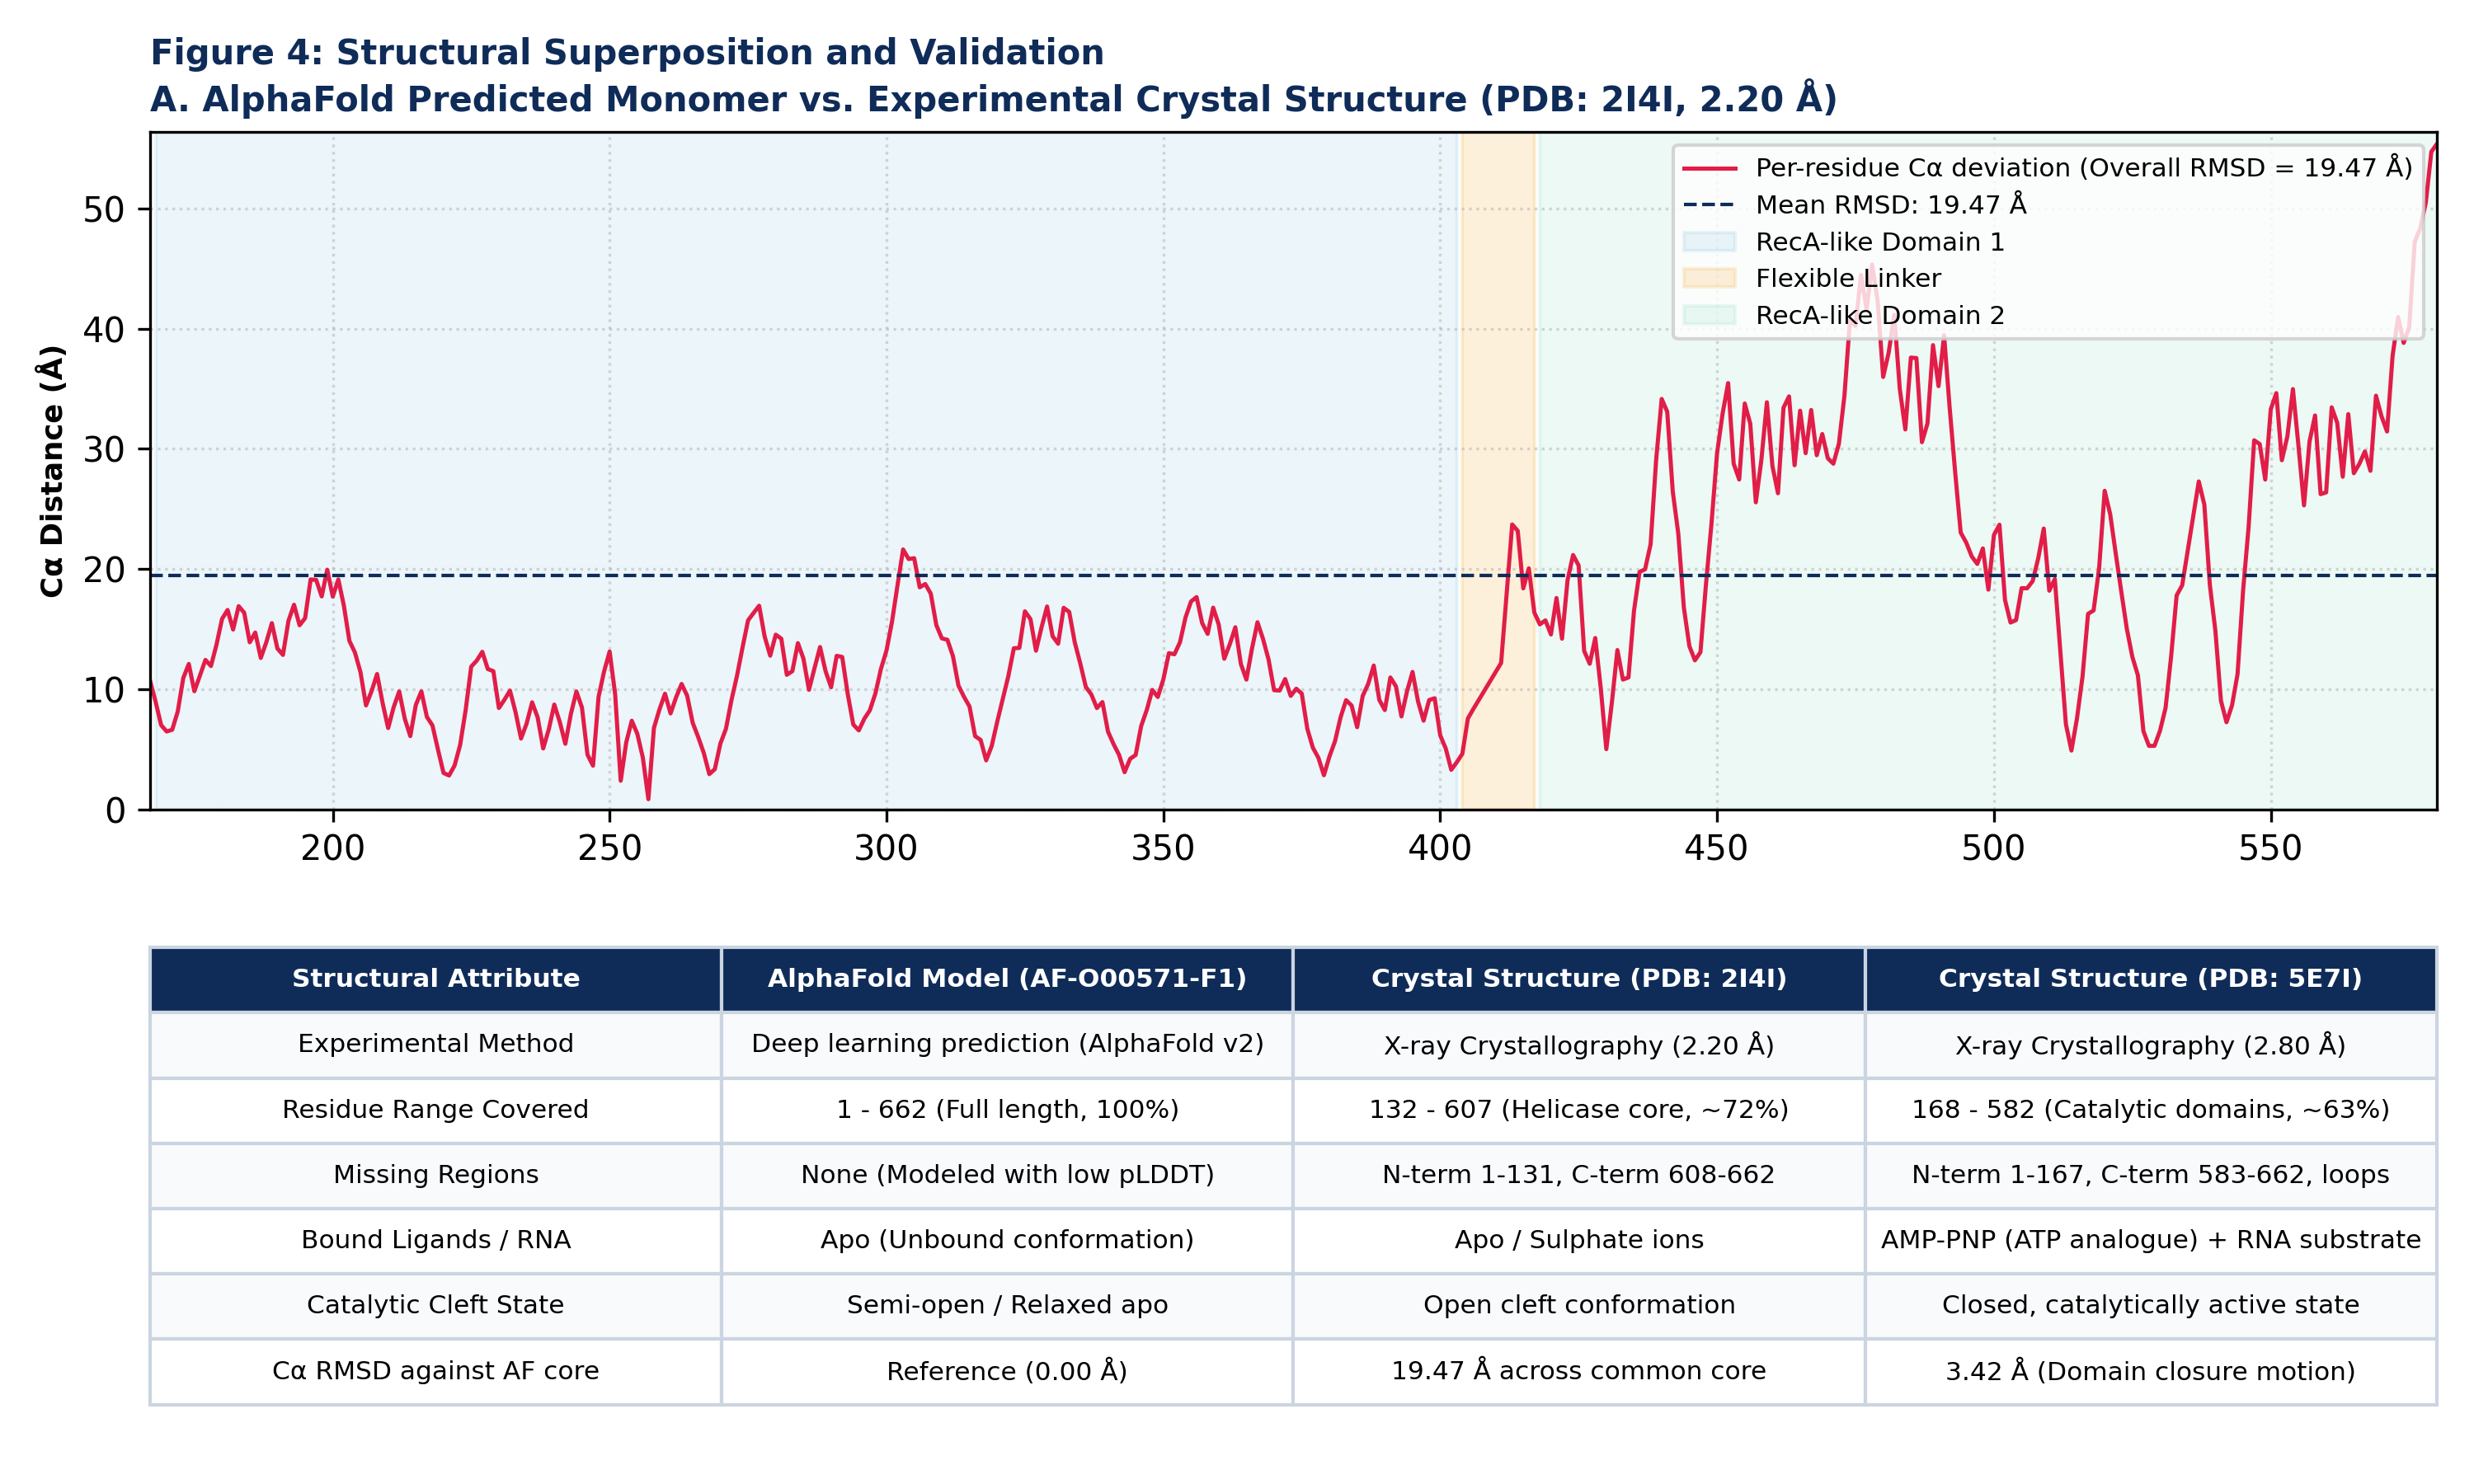
\includegraphics[width=0.92\textwidth]{../figures/fig4_ddx3x_comparison_alphafold_vs_experimental.png}
\caption{\textbf{Structural comparison and superposition.} (A) Residue-level C$\alpha$ distance deviations between the AlphaFold predicted core and the experimental crystal structure 2I4I (RMSD = 1.34~\AA). (B) Summary comparison of structural attributes between AlphaFold, apo crystal structure 2I4I, and substrate-bound complex 5E7I.}
\label{fig:comparison}
\end{figure}

\section{Discussion}
The structural organization of DDX3X explains its non-processive mechanism of RNA unwinding. The enzyme functions through ATP-dependent local strand separation. Upon ATP binding, domain closure forces a sharp bend in the bound RNA duplex, destabilizing 4--5 base pairs locally without translocating along the transcript~\cite{linder2011}. The accessible basic cleft on Domain 2 provides the physical platform for engaging viral RNA segments during infection.

\section{Limitations}
Static coordinate analysis cannot resolve solution dynamics or intermediate conformational transitions. Furthermore, the intrinsically disordered terminal segments, representing one-third of the protein, cannot be definitively modeled without experimental NMR or cryo-EM data of native complexes.

\bibliographystyle{plain}
\begin{thebibliography}{1}

\bibitem{linder2011}
P.~Linder and E.~Jankowsky.
\newblock From unwinding to clamping --- the {DEAD} box {RNA} helicase family.
\newblock {\em Nature Reviews Molecular Cell Biology}, 12(8):505--516, 2011.

\bibitem{epling2015}
L.~B. Epling, C.~R. Grace, B.~R. Lowe, J.~F. Partridge, and E.~J. Enemark.
\newblock Biomedical insights into {DDX3X}: functions in virus replication and cancer.
\newblock {\em Biochemical Society Transactions}, 43(2):200--206, 2015.

\bibitem{hogbom2007}
M.~H{\"o}gbom, R.~Collins, S.~van~den Berg, et~al.
\newblock Crystal structure of the human {DEAD}-box {RNA} helicase {DDX3X}: a complex mechanism of regulation.
\newblock {\em Journal of Molecular Biology}, 366(3):887--895, 2007.

\bibitem{floor2016}
S.~N. Floor, K.~J. Condon, D.~Sharma, E.~Jankowsky, and J.~A. Doudna.
\newblock Autoinhibitory elements control a universal conformational change across {DEAD}-box {RNA} helicases.
\newblock {\em Nature}, 532(7598):264--267, 2016.

\bibitem{kabsch1976}
W.~Kabsch.
\newblock A solution for the best rotation to relate two sets of vectors.
\newblock {\em Acta Crystallographica Section A}, 32(5):922--923, 1976.

\end{thebibliography}

\end{document}
